\section{Газовые законы}
%TODO Время удара футбольного мяча

\begin{ex} 
(2001) Какой максимальной температуры достигнет 1 моль идеального газа в процессе, изображенном на рисунке? 
\begin{center}
\begin{tikzpicture}
	\draw[arrows={-latex}] (0,0) -- (3,0) node[above] {$V$};
	\draw[arrows={-latex}] (0,0) -- (0,3) node[right] {$p$};
	%\draw (0,0) circle (2pt)
	\coordinate [label=left:{$p_0$}] (A) at (0,2.5);
	\coordinate [label=below	:{$V_0$}] (B) at (2.5,0);
	\draw plot[raw gnuplot, smooth] function{set xrange[0.2:2.3]; plot 2.5-x lt 2};
\end{tikzpicture}
\end{center}
\begin{ans}
$T_{\max}=p_0V_0/(4R)$
\end{ans}
\end{ex}

\begin{ex}
Найдите максимальную температуру идеального газа в процессе, протекающем по закону $P=P_0~-~\alpha~V^2$, где $P_0$ и $\alpha$ -- положительные постоянные, $V$ -- объем одного моля.
\begin{ans}
$T_{\max} = \sqrt{p_0/3\alpha}$
\end{ans}
\end{ex}

\begin{ex}
(2010) Посередине откаченной и запаянной с обоих концов горизонтально расположенной трубки длины $L$ находится столбик ртути длины $h$. 
Если трубку поставить вертикально, столбик ртути смеситься на расстояние $x$. Какое первоначальное давление в трубке? Плотность ртути $\rho$.
\begin{ans}
$p_0 = \rho g h \left( (L-h)^2 - 4x^2 \right)/ (4x(L-h))$
\end{ans}
\end{ex}

\begin{ex}
(2013) В баллон, вместимостью $V$, при давлении $p$ нагнетают воздух. За какое время $t$ он будет накачан до давления $p_n$, если компрессор за время $\tau$ засасывает объем $V_0$ атмосферного воздуха? 
Температуру считать неизменной, а атмосферное давление равным $p_0$. Как изменится ответ, если воздух откачивать из баллона?
\begin{ans}
$t_1 = \tau V(p_n-p)/(p_0V_0)$, $t_2 = \tau \log p/p_n /\log (1+V_0/V)$
\end{ans}
\end{ex}

\begin{ex}
\hspace{0pt} \\
\begin{minipage}{.65\textwidth}
(2012) На поверхности жидкости плотностью $\rho$ плавает тонкостенный цилиндрический стакан высотой $h$, наполовину погруженный в жидкость. 
На какую глубину $h_1$ погрузится стакан в жидкость, если его осторожно положить на поверхность жидкости вверх дном? 
На какую глубину $h_2$ нужно утопить перевернутый вверх дном стакан, чтобы он вместе с заключенным в нем воздухом пошел ко дну? Давление атмосферы $p_0$.
\end{minipage}
\begin{minipage}{.35\textwidth}
\centering
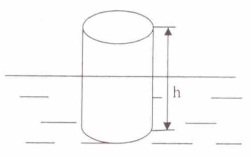
\includegraphics[width = 0.9 \textwidth]{082012GasLawsGlass.jpg}
\end{minipage}
\begin{ans}
$h_1 = h \frac{2p_0+3\rho gh}{2(2p_0 + \rho gh)}$
\end{ans}
\end{ex}

\begin{ex}
\hspace{0pt} \\
\begin{minipage}{.65\textwidth}
В вертикальном закрытом сосуде имеется поршень, который может перемещаться без трения. 
По обе стороны от поршня находятся одинаковые массы одного и того же газа. 
При температуре $T$ объем верхней части в $n$ раз больше, чем объем нижней. 
Каким будет соотношение этих объемов, если повысить температуру до значения $T_2$?
\end{minipage}
\begin{minipage}{.35\textwidth}
\centering
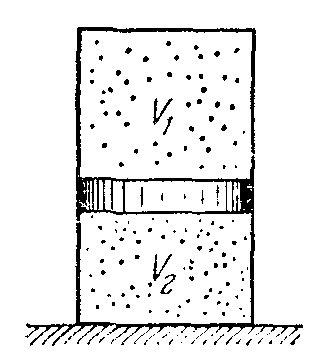
\includegraphics[width = 0.75 \textwidth]{0805GasLawsPiston.jpg}
\end{minipage}
\begin{ans}
\end{ans}
\end{ex}

\section{Молекулярно-кинетическая теория}

%Ижевск
\begin{ex}
\hspace{0pt} \\
\begin{minipage}{.65\textwidth}
Два сосуда одинакового объема соединены трубками. Диаметр одной из трубок велик, 
а другой мал по сравнению со средней длиной свободного пробега молекул газа, находящегося в сосуде. 
Первый сосуд поддерживается при температуре $T$, а второй при температуре $4T$. 
В каком направлении будет перетекать газ по узкой трубке, если перекрыть широкую трубку? 
Какая масса газа перейдет при этом из одного сосуд в другой, если общая масса газа в обоих сосудах равна $M$?
\end{minipage}
\begin{minipage}{.35\textwidth}
\centering
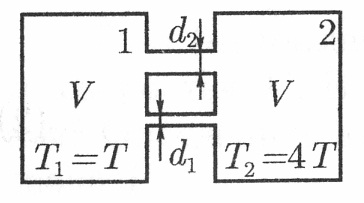
\includegraphics[width = 0.9 \textwidth]{0806KineticTheoryTwoVessels.jpg}
\end{minipage}
\begin{ans}
\end{ans}
\end{ex}

%Ижевск
\begin{ex}
\hspace{0pt} \\
\begin{minipage}{.65\textwidth}
Теплоизолированная полость небольшими малыми одинаковыми отверстиями соединена с двумя объемами, содержащими газообразный гелий. 
Давления в этих объемах поддерживаются одинаковыми и равными $P$, а температуры поддерживаются равными в одном из объемов $T$, в другом $2T$. 
Найдите установившиеся давление и температуру внутри полости.
\end{minipage}
\begin{minipage}{.35\textwidth}
\centering
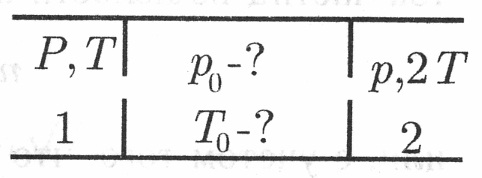
\includegraphics[width = 0.9 \textwidth]{0807KineticTheoryHelium.jpg}
\end{minipage}
\begin{ans}
\end{ans}
\end{ex}

%Черепанов
\begin{ex}
Плоская поверхность нагрета неравномерно, так что вдоль нее поддерживается градиент температуры $dT/dx$. 
В этих условиях газ, примыкающий к поверхности, приходит в движение вдоль поверхности. Это явление называют тепловым скольжением. 
Объясните его механизм и оцените скорость теплового скольжения. Необходимые параметры считать известными.
\begin{ans}
\end{ans}
\end{ex}

\begin{ex}
(2008) Оценить по порядку величины установившуюся скорость, с которой будет двигаться в сильно разреженном воздухе плоский диск, одна из сторон которого нагрета до температуры $T_1$, а другая до температуры $T_2$, $T_1>T_2$. Температура воздуха равна $T$.
\begin{ans}
\end{ans}
\end{ex}

\begin{ex}
(2009) Каково должно быть максимальное значение температурного градиента $dT/dz$ атмосферного воздуха, 
чтобы он мог находиться в устойчивом механическом равновесии? Воздух считать двухатомным газом с относительной молекулярной массой $\mu$. 
Ускорение свободного падения $g$ не зависит от высоты над поверхностью земли.
\begin{ans}
\end{ans}
\end{ex}